\documentclass[preprint,12pt,authoryear]{elsarticle}
\biboptions{authoryear,round,semicolon}
% \citet{smith2020}  % Smith (2020)
% \citep{smith2020}  % (Smith, 2020)



\usepackage[english]{babel}
\usepackage{amssymb,amsmath,amsfonts,amsthm}
\usepackage[most]{tcolorbox}
\newtheorem{lemma}{Lemma}
\usepackage{threeparttable}
\usepackage{xcolor}
\usepackage{longtable}
\usepackage{url}
\usepackage{multirow}
\usepackage{soul}
\usepackage{xcolor}
\usepackage{bbm}
\usepackage[most]{tcolorbox}
\usepackage{amsmath, amssymb}

\usepackage{soul}
\usepackage{adjustbox}
\usepackage{booktabs}
\usepackage{makecell}
\usepackage{threeparttable}
\usepackage{graphicx}
\usepackage{array}
\usepackage{float}
\usepackage[utf8]{inputenc}
\usepackage[T1]{fontenc}
\usepackage{hyperref}
\usepackage[top=2.5cm, bottom=2.5cm, left=3cm, right=2.5cm]{geometry}

\usepackage{tikz}
\usetikzlibrary{arrows.meta, positioning, decorations.pathreplacing, shapes.geometric}
\usepackage{graphicx} 


\journal{Journal XYZ}

\hypersetup{
    colorlinks=true,
    allcolors=black
}


\begin{document}

% Define a custom highlight box
\tcbset{highlight/.style={colback=yellow!25!white, colframe=yellow!75!black, 
    sharp corners, boxrule=0.5mm, width=\textwidth, enlarge left by=-5mm, 
    enlarge right by=-5mm}}

\begin{frontmatter}

% Title & Authors
\title{Partisanship and Inflation Perceptions: Evidence from Michigan, 2019–2024}

\author[1]{NaN\corref{cor1}
}
\ead{email}



\address[1]{NaN}




\begin{abstract}
This paper analyzes determinants of inflation perceptions among 1,000 Michigan residents surveyed in 2024, in the run-up to the U.S. presidential election. Ordered logistic regressions show that political leaning is the strongest predictor: Republicans and Independents perceive significantly higher inflation than Democrats, and Trump supporters and Biden administration disapprovers report sharply higher inflation than Harris supporters or those with positive approval. Gender differences are also robust, with women more likely than men to report higher inflation across all domains. By contrast, age, income, education, and rural–urban location have weaker or inconsistent effects, while home ownership consistently dampens perceptions of inflation, particularly in housing and gasoline. These findings highlight that perceptions of inflation are politicized and gendered, reflecting partisan and leadership evaluations more than local economic fundamentals.

\end{abstract}


\begin{keyword}
Inflation perceptions, Partisanship, Leader approval, Voting intention
\end{keyword}

\end{frontmatter}

\newpage


\section{Introduction}

Inflation perceptions have become increasingly politicized in recent years, especially in battleground states such as Michigan. While official statistics document price dynamics, what matters for political behavior is how individuals perceive these changes. Prior research shows that partisan identity often colors economic perceptions, yet less is known about how local economic context and demographics intersect with these political divides. We address this gap with a survey of 1,000 Michigan residents conducted in 2024, asking respondents how they perceived price changes over the past five years. We analyze the drivers of these perceptions, with attention to partisanship, presidential vote choice, gender, and county-level economic conditions.

\section{Inflation as a Political Issue}
Inflation is not only an economic statistic. It is a lived, frequently discussed experience that shapes how citizens judge governments and parties. People encounter prices at the pump, the grocery aisle, and in rent, so they form views quickly and often with limited information. These views travel through media narratives and partisan discussion networks, which means perceptions can diverge from official indices and from each other.

\begin{itemize}
    \item PAPERS on political psychology on motivated reasoning and economic perceptions
\end{itemize}


\section{Democratic Accountability and Biased Perceptions }

Classic accounts of democratic accountability assume that voters reward or punish incumbents for economic performance that they observe with reasonable accuracy.

\begin{itemize}
    \item PAPERS on economic voting and partisan motivated reasoning
\end{itemize}




\section{Michigan as a Strategic Case}
Michigan serves as a compelling case study for how inflation perceptions intersect with political dynamics. As a competitive swing state, even small shifts in attitudes toward prices can tip statewide outcomes. The state’s economy is diverse: industrial and logistics corridors in the south contrast with tourism and service-oriented counties in the north. This variety produces different price environments, commuting patterns, and media markets, all of which shape how residents both experience and interpret inflation.

Michigan’s strategic importance is further magnified by its growing role in presidential primaries. As of mid-2025, the Democratic Party is weighing Michigan as one of the earliest states in the 2028 primary schedule. Representative Debbie Dingell, who sits on the committee deciding the order, stressed that whichever state goes first draws disproportionate campaign attention, candidate visits, and national media focus. Should Michigan secure this position, it would become not just a swing state but a bellwether of campaign messaging—where inflation and cost-of-living concerns are likely to be spotlighted at the very outset of the national political calendar.

Taken together, Michigan’s economic heterogeneity, households’ lived cost pressures, partisan political framing, and rising importance in national party strategy make it an especially instructive microcosm. It is a site where local economic structures, everyday struggles, and partisan identity interact, shaping both perceptions of inflation and their potential political consequences.


\section{Survey}

We collected original data on inflation perceptions using the State of the State Survey (SOSS), a long-running public opinion survey conducted by the Institute for Public Policy and Social Research (IPPSR) at Michigan State University.\footnote{https://ippsr.msu.edu/survey-research/state-state-survey-soss/soss-data} The SOSS has been widely used by scholars and policymakers to track public opinion in Michigan, and it provides a reliable platform for measuring political and economic attitudes. For this project, our survey module was fielded between September 23 and October 10, 2024.

The survey relied on a mixed-mode design that combined online and phone interviews. This approach was adopted to reach respondents across different demographic and geographic groups. Online interviews are more effective for younger and urban residents, while phone interviews are useful for older participants and those living in rural areas. In total, 1,174 Michigan adults participated in the survey. The survey firm then used post-stratification matching to produce a final dataset of 1,000 respondents. This step ensured balance across age, gender, race, and region, thereby enhancing the representativeness of the sample.

The survey module addressed three guiding questions. First, to what extent do political factors such as partisan identity, presidential approval, and 2024 vote intention shape perceptions of inflation relative to demographic and household characteristics? Second, do these political and demographic influences vary across domains of everyday consumption—restaurants, groceries, housing, and gasoline—or do they follow a consistent pattern across categories? Third, what do these results imply for democratic accountability, particularly whether citizens’ inflation perceptions are tied more to partisan and leadership evaluations than to underlying economic condition

\section{Results}
Our dependent variables measure perceived price changes across five domains: overall prices, restaurant meals, groceries, housing, and gasoline. Respondents were asked: “Compared with five years ago, is the price lower, the same, a little higher, or a lot higher?” with five response categories. We drop “Don’t know/Not sure” responses from the analysis, leaving a four-category ordered outcome where higher values correspond to higher perceived inflation.

Because these responses are naturally ordered but not continuous, we estimate ordered logistic regression models. Ordered logit is appropriate when the dependent variable reflects a ranking of outcomes, as in this case from “lower” to “a lot higher,” but the distance between categories cannot be assumed equal. The model estimates the log-odds of being in a higher perception category relative to all lower categories, under the proportional odds assumption. To aid interpretation, we report exponentiated coefficients as odds ratios. An odds ratio greater than one indicates that the predictor increases the likelihood of perceiving higher inflation, while an odds ratio below one indicates a lower likelihood. Cutpoints are reported at the bottom of the tables and capture the thresholds between categories.

Table~\ref{tab:main} compares three specifications using overall price perceptions as the dependent variable. Political variables dominate across models. In the partisan identity model shown in column (1), Republicans report much higher perceived inflation than Democrats, with an odds ratio of 7.03 ($p<0.01$). Independents and others also report higher inflation than Democrats, with an odds ratio of 2.40 ($p<0.01$). Substituting presidential job approval raises explanatory power. In column (2), relative to respondents rating the Biden administration as "Excellent," those reporting "Poor" approval have 16.98 times the odds of perceiving higher inflation ($p<0.01$), while those rating "Fair" have 4.03 times the odds ($p<0.01$). Vote intentions for 2024 presidential election show a similar structure. As shown in column (3), Trump supporters report 10.22 times the odds of perceiving higher inflation than Harris supporters ($p<0.01$), and other candidate supporters report 2.96 times the odds ($p<0.01$).  

Demographic controls show smaller but consistent associations. Women are more likely than men to report higher inflation across all specifications, with odds ratios between 1.71 and 1.90 ($p<0.01$). Home ownership is associated with lower perceived inflation (OR = 0.72 to 0.79, $p\leq 0.10$). Age has a small convex pattern: the linear term is positive and significant in some models, while the squared term is close to one, suggesting only a weak nonlinearity. Income, education, and rural--urban status show inconsistent effects.  

Model fit improves once leader approval and vote choice are included. The pseudo-$R^2$ rises from 0.093 in the partisan identity model to 0.182 in the job approval model and 0.152 in the vote intention model. This suggests that leader evaluations and prospective choices capture much of the politicization of inflation perceptions.  



\begin{center}
\textbf{TABLE 1 AROUND HERE}
\end{center}

Tables~\ref{tab:pol}--\ref{tab:vot} repeat the analysis across four item categories. The politicization of perceptions is evident in every category but is strongest for groceries and gasoline. In the partisan model, Republicans are nearly six times as likely as Democrats to perceive higher grocery prices (OR = 5.90, $p<0.01$) and more than eight times as likely to perceive higher gasoline prices (OR = 8.47, $p<0.01$). Similar gaps appear in the job approval and vote intention models, with particularly large coefficients for gas. These results indicate that frequently purchased and highly visible goods are most susceptible to partisan framing.  

Housing perceptions show a somewhat different pattern. Although Republicans and Trump supporters still report higher inflation, home ownership strongly reduces perceived housing inflation (OR = 0.43 to 0.45, $p<0.01$). People who own their homes are less likely to say housing costs have gone up, which suggests that owning a home shields them from feeling price increases in the housing market. This pattern is consistent with research showing that home ownership provides a degree of insulation from price increases. Homeowners with fixed-rate mortgages face stable monthly payments and are not directly exposed to rent hikes, so they often perceive less inflation in housing (CITE). By contrast, renters experience inflation more directly as rents adjust at lease renewal, which helps explain their higher sensitivity (CITE). At the same time, homeowners may benefit from viewing their property as a hedge against inflation, reinforcing the perception that they are less vulnerable to rising housing costs.

Gender gaps are consistent across categories. Women report higher perceived inflation in restaurants, groceries, housing, and gasoline, with odds ratios between 1.4 and 2.2 ($p<0.01$). This finding aligns with prior work showing that women systematically perceive or expect higher inflation than men, even after controlling for demographic and socioeconomic factors (CITE). One explanation is differential exposure among them. Women are often more involved in household purchasing, particularly for groceries and other frequently bought goods, which increases the salience of rising prices (CITE). These patterns suggest that inflation perceptions are not only politicized but also gendered, reflecting systematic differences in how men and women experience and interpret price changes. 

Age, income, and education again have limited or inconsistent effects, with the exception that middle-income households between 60 thousand dollars to 99 thousand dollars perceive lower gasoline inflation than lower-income households. 

\begin{center}
\textbf{TABLE 2-4 AROUND HERE}
\end{center}

Taken together, the results indicate that inflation perceptions in Michigan are politicized and gendered. Political affiliation, leader approval, and vote choice are the most consistent predictors, while local economic fundamentals and standard demographics explain relatively little. Housing stands out as the one domain where economic position, specifically home ownership, exerts a strong protective effect. Gasoline and groceries, by contrast, are categories where political divisions are most visible. The overall pattern suggests that evaluations of government performance and partisan loyalties filter how citizens interpret price changes, raising questions about the role of economic reality in democratic accountability.  



\section{Discussion}
Our findings show that inflation perceptions in Michigan are strongly politicized. Partisan identity, presidential approval, and vote intention are the most powerful predictors, with leader approval in particular producing very large differences. This aligns with research on motivated reasoning in economic perceptions (CITE). Demographic effects are smaller but consistent. Women report higher perceived inflation across all domains, echoing prior evidence of a gender gap in inflation perceptions. Home ownership reduces perceptions of rising housing costs, likely because owners are shielded from rent increases and benefit from fixed mortgage payments.

Together, these results suggest that inflation perceptions are shaped less by local economic fundamentals and more by political and social identities. This politicization complicates democratic accountability, as judgments of government performance may depend as much on partisan cues and household circumstances as on actual price dynamics.


% no appendix header/lettering
\clearpage
\phantomsection
\section*{Tables}
\addcontentsline{toc}{section}{Tables} 
\label{sec:tables}

\begin{table}[H]
\centering
\caption{Model 3}
\label{tab:Model3}
\renewcommand{\arraystretch}{1.1}
\begin{tabular}{lccc}
\hline
\hline
\textbf{Variable} & \textbf{Coef.} & \textbf{z} & \textbf{P>|z|} \\
\hline
$\mu$ & 2.195 & 20.88 & 0.000 \\
Urban                & 0.001 & 0.09  & 0.930 \\
Weighted Tax                 & 0.023 & 7.38  & 0.000 \\
Distance to Refinery  & 0.00018 & 9.21 & 0.000 \\
Distance to Terminal  & 0.00064 & 16.73 & 0.000 \\
Reformulated Fuel (RFG)      & 0.009 & 1.12  & 0.264 \\
Population          & 2.29e-08 & 4.48 & 0.000 \\
Mean Temperature             & -0.00165 & -48.24 & 0.000 \\
January   & 0.355 & 435.74 & 0.000 \\
February  & 0.346 & 570.37 & 0.000 \\
March     & 0.455 & 665.49 & 0.000 \\
April     & 0.584 & 699.88 & 0.000 \\
May       & 0.629 & 573.76 & 0.000 \\
June      & 0.491 & 373.73 & 0.000 \\
July      & 0.538 & 383.56 & 0.000 \\
August    & 0.433 & 316.97 & 0.000 \\
September & 0.248 & 204.59 & 0.000 \\
October   & 0.179 & 185.17 & 0.000 \\
November  & 0.045 & 58.83  & 0.000 \\
Year 2025 & -0.332 & -861.90 & 0.000 \\
\hline
\hline
\multicolumn{4}{c}{\textbf{Random Effects Parameters}} \\
\hline
\textbf{Group (Parameter)} & \textbf{SD Model 3} & \textbf{SD Model 0} & \textbf{Var. (\%)} \\
\hline
State (urban2 slope)        & 0.0074551 & --       & --     \\
State ($\sigma_s^2$)        & 0.0520408 & 0,0456562    & \textbf{-14\%} \\
County ($\sigma_c^2$)       & 0.006531  & 0,0072391   & \textbf{-10\%} \\
Station ID ($\sigma_j^2$)   & 0.0189879 & 0,0189889   & \textbf{0\%} \\
Residual ($\sigma_{i}^2$)   & 0.0185978 & 0,0185978   & \textbf{0\%} \\
Total variance ($\sigma_s^2+\sigma_c^2+\sigma_j^2+\sigma_{i}^2$) & 0,1036126 & 0,090482&\textbf{15\%} \\
\hline
\hline
\multicolumn{4}{c}{\textbf{Variance Attribution by Spatial Level}} \\
\hline
\textbf{Level} & \textbf{ICC} & \textbf{SE} & \textbf{Var. (\%)} \\
\hline
State                     & 0.540 & 0.051 & \textbf{57\%} \\
County\,|\,State          & 0.610 & 0.043 & \textbf{6\%} \\
Station\,|\,County\,|\,State & 0.800 & 0.021 & \textbf{18}\% \\
Month\,|\, Station\,|\,County\,|\,State & NA & NA  & \textbf{18\%} \\
\hline
\hline
\end{tabular}

\vspace{1em}
\raggedright
\scriptsize
\textit{Note: The ICC is reported in its cumulative form, reflecting the proportion of total variance attributable to each level up to that point in the hierarchy.}
\end{table}


% \clearpage
% \phantomsection
% \section*{Figures}
% \addcontentsline{toc}{section}{Figures} % optional
% \label{sec:figures}
% \begin{figure}[H]
\centering
\begin{tcolorbox}[colback=white, colframe=black, boxrule=0.4pt, arc=2pt, left=2mm, right=2mm, top=1mm, bottom=1mm]
\begin{center}
\resizebox{0.8\textwidth}{!}{
  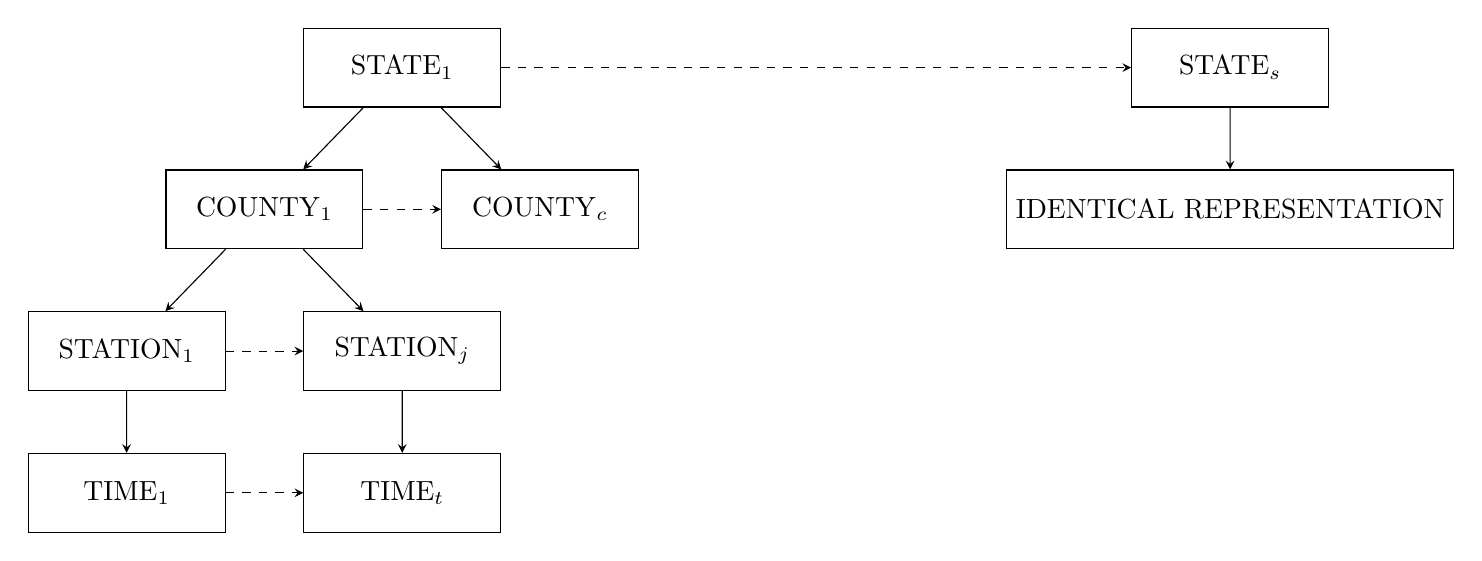
\begin{tikzpicture}[
    every node/.style={draw, minimum width=2.5cm, minimum height=1cm, font=\sffamily},
    level distance=1.8cm,
    sibling distance=3.5cm,
    ->, >=stealth
  ]

  % Nodos
  \node (state1) {$\mathrm{STATE}_{1}$}
    child {node (county1) {$\mathrm{COUNTY}_{1}$} 
      child {node (station1) {$\mathrm{STATION}_{1}$}
        child {node (time1) {$\mathrm{TIME}_{1}$}}
      }
      child {node (stationk) {$\mathrm{STATION}_{j}$}
        child {node (timet) {$\mathrm{TIME}_{t}$}}
      }
    }
    child {node (countyc) {$\mathrm{COUNTY}_{c}$}};

  \node[right=8cm of state1] (statez) {$\mathrm{STATE}_{s}$}
    child {node (others) {$\mathrm{IDENTICAL\ REPRESENTATION}$}};

  \draw[dashed] (county1) -- (countyc);
  \draw[dashed] (station1) -- (stationk);
  \draw[dashed] (time1) -- (timet);
  \draw[dashed] (state1) -- (statez);

  \end{tikzpicture}
}
\end{center}
\end{tcolorbox}
\caption{Hierarchical structure of the multilevel model: states, counties, stations, and time.}
\label{fig:hierarchy}
\end{figure}


\begin{figure}[h]
    \centering
    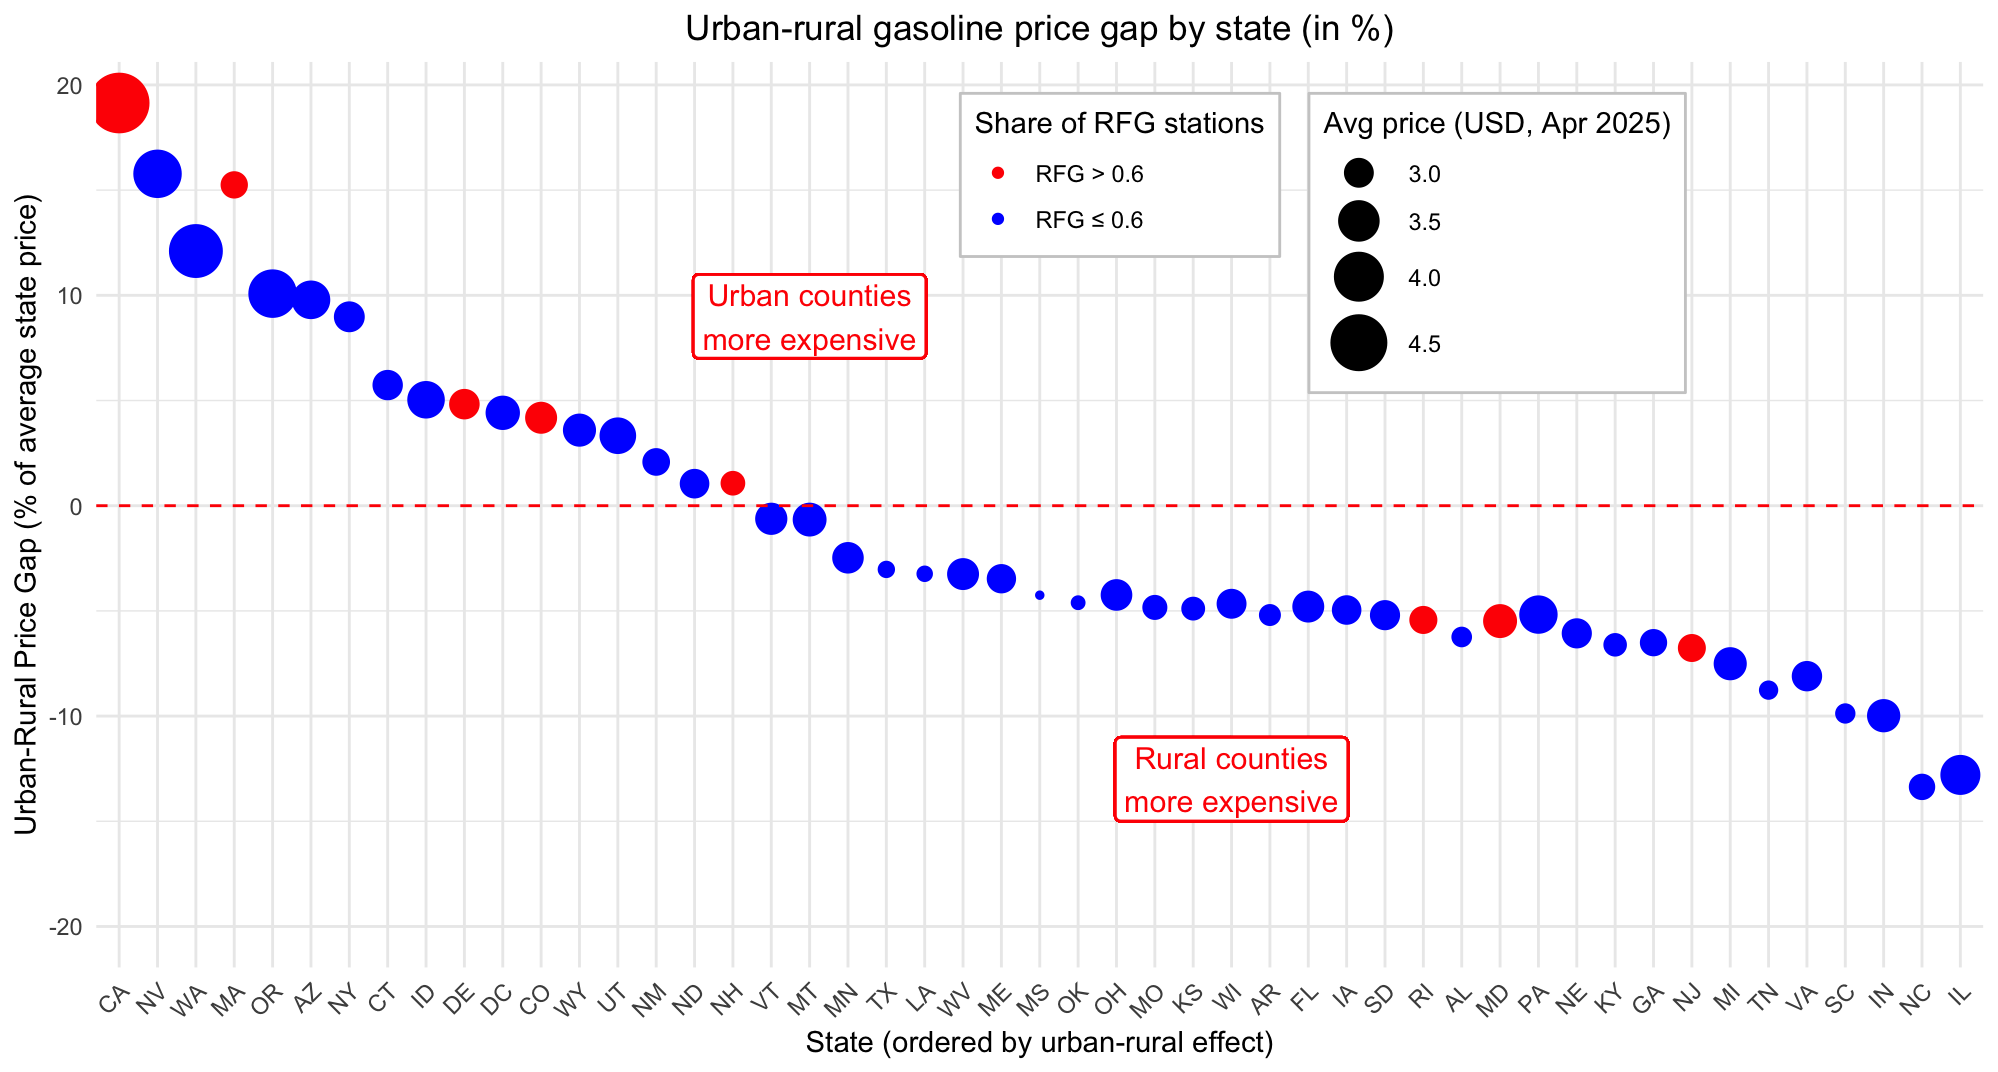
\includegraphics[width=\linewidth]{Figures/Rplot02.png}
\caption{State-Level Urban–Rural Gasoline Price Gaps (as Percentage of State Average)}

    \label{fig:Figure2}
\end{figure}

\newpage

% \appendix
% \clearpage

% \section{Tables}
% 
\begin{table}[H]
\centering
\caption{Model 3}
\label{tab:Model3}
\renewcommand{\arraystretch}{1.1}
\begin{tabular}{lccc}
\hline
\hline
\textbf{Variable} & \textbf{Coef.} & \textbf{z} & \textbf{P>|z|} \\
\hline
$\mu$ & 2.195 & 20.88 & 0.000 \\
Urban                & 0.001 & 0.09  & 0.930 \\
Weighted Tax                 & 0.023 & 7.38  & 0.000 \\
Distance to Refinery  & 0.00018 & 9.21 & 0.000 \\
Distance to Terminal  & 0.00064 & 16.73 & 0.000 \\
Reformulated Fuel (RFG)      & 0.009 & 1.12  & 0.264 \\
Population          & 2.29e-08 & 4.48 & 0.000 \\
Mean Temperature             & -0.00165 & -48.24 & 0.000 \\
January   & 0.355 & 435.74 & 0.000 \\
February  & 0.346 & 570.37 & 0.000 \\
March     & 0.455 & 665.49 & 0.000 \\
April     & 0.584 & 699.88 & 0.000 \\
May       & 0.629 & 573.76 & 0.000 \\
June      & 0.491 & 373.73 & 0.000 \\
July      & 0.538 & 383.56 & 0.000 \\
August    & 0.433 & 316.97 & 0.000 \\
September & 0.248 & 204.59 & 0.000 \\
October   & 0.179 & 185.17 & 0.000 \\
November  & 0.045 & 58.83  & 0.000 \\
Year 2025 & -0.332 & -861.90 & 0.000 \\
\hline
\hline
\multicolumn{4}{c}{\textbf{Random Effects Parameters}} \\
\hline
\textbf{Group (Parameter)} & \textbf{SD Model 3} & \textbf{SD Model 0} & \textbf{Var. (\%)} \\
\hline
State (urban2 slope)        & 0.0074551 & --       & --     \\
State ($\sigma_s^2$)        & 0.0520408 & 0,0456562    & \textbf{-14\%} \\
County ($\sigma_c^2$)       & 0.006531  & 0,0072391   & \textbf{-10\%} \\
Station ID ($\sigma_j^2$)   & 0.0189879 & 0,0189889   & \textbf{0\%} \\
Residual ($\sigma_{i}^2$)   & 0.0185978 & 0,0185978   & \textbf{0\%} \\
Total variance ($\sigma_s^2+\sigma_c^2+\sigma_j^2+\sigma_{i}^2$) & 0,1036126 & 0,090482&\textbf{15\%} \\
\hline
\hline
\multicolumn{4}{c}{\textbf{Variance Attribution by Spatial Level}} \\
\hline
\textbf{Level} & \textbf{ICC} & \textbf{SE} & \textbf{Var. (\%)} \\
\hline
State                     & 0.540 & 0.051 & \textbf{57\%} \\
County\,|\,State          & 0.610 & 0.043 & \textbf{6\%} \\
Station\,|\,County\,|\,State & 0.800 & 0.021 & \textbf{18}\% \\
Month\,|\, Station\,|\,County\,|\,State & NA & NA  & \textbf{18\%} \\
\hline
\hline
\end{tabular}

\vspace{1em}
\raggedright
\scriptsize
\textit{Note: The ICC is reported in its cumulative form, reflecting the proportion of total variance attributable to each level up to that point in the hierarchy.}
\end{table}

% \label{table}

% \clearpage
% \section{Figures}
% \begin{figure}[H]
\centering
\begin{tcolorbox}[colback=white, colframe=black, boxrule=0.4pt, arc=2pt, left=2mm, right=2mm, top=1mm, bottom=1mm]
\begin{center}
\resizebox{0.8\textwidth}{!}{
  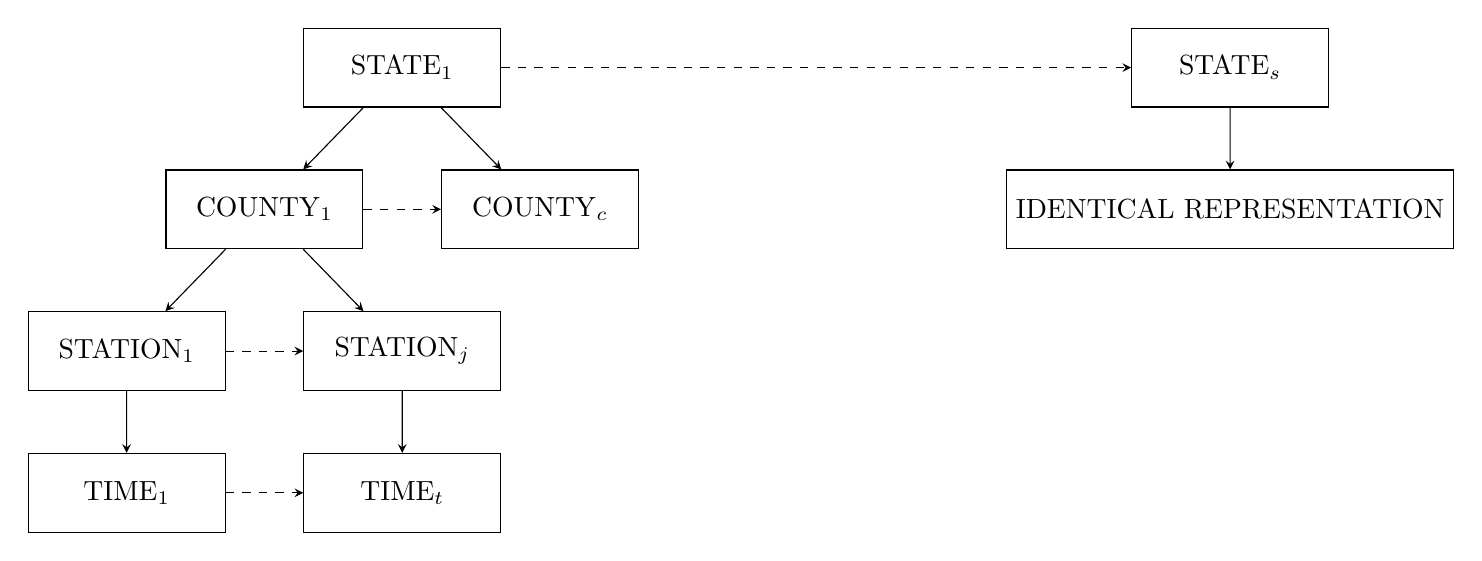
\begin{tikzpicture}[
    every node/.style={draw, minimum width=2.5cm, minimum height=1cm, font=\sffamily},
    level distance=1.8cm,
    sibling distance=3.5cm,
    ->, >=stealth
  ]

  % Nodos
  \node (state1) {$\mathrm{STATE}_{1}$}
    child {node (county1) {$\mathrm{COUNTY}_{1}$} 
      child {node (station1) {$\mathrm{STATION}_{1}$}
        child {node (time1) {$\mathrm{TIME}_{1}$}}
      }
      child {node (stationk) {$\mathrm{STATION}_{j}$}
        child {node (timet) {$\mathrm{TIME}_{t}$}}
      }
    }
    child {node (countyc) {$\mathrm{COUNTY}_{c}$}};

  \node[right=8cm of state1] (statez) {$\mathrm{STATE}_{s}$}
    child {node (others) {$\mathrm{IDENTICAL\ REPRESENTATION}$}};

  \draw[dashed] (county1) -- (countyc);
  \draw[dashed] (station1) -- (stationk);
  \draw[dashed] (time1) -- (timet);
  \draw[dashed] (state1) -- (statez);

  \end{tikzpicture}
}
\end{center}
\end{tcolorbox}
\caption{Hierarchical structure of the multilevel model: states, counties, stations, and time.}
\label{fig:hierarchy}
\end{figure}


\begin{figure}[h]
    \centering
    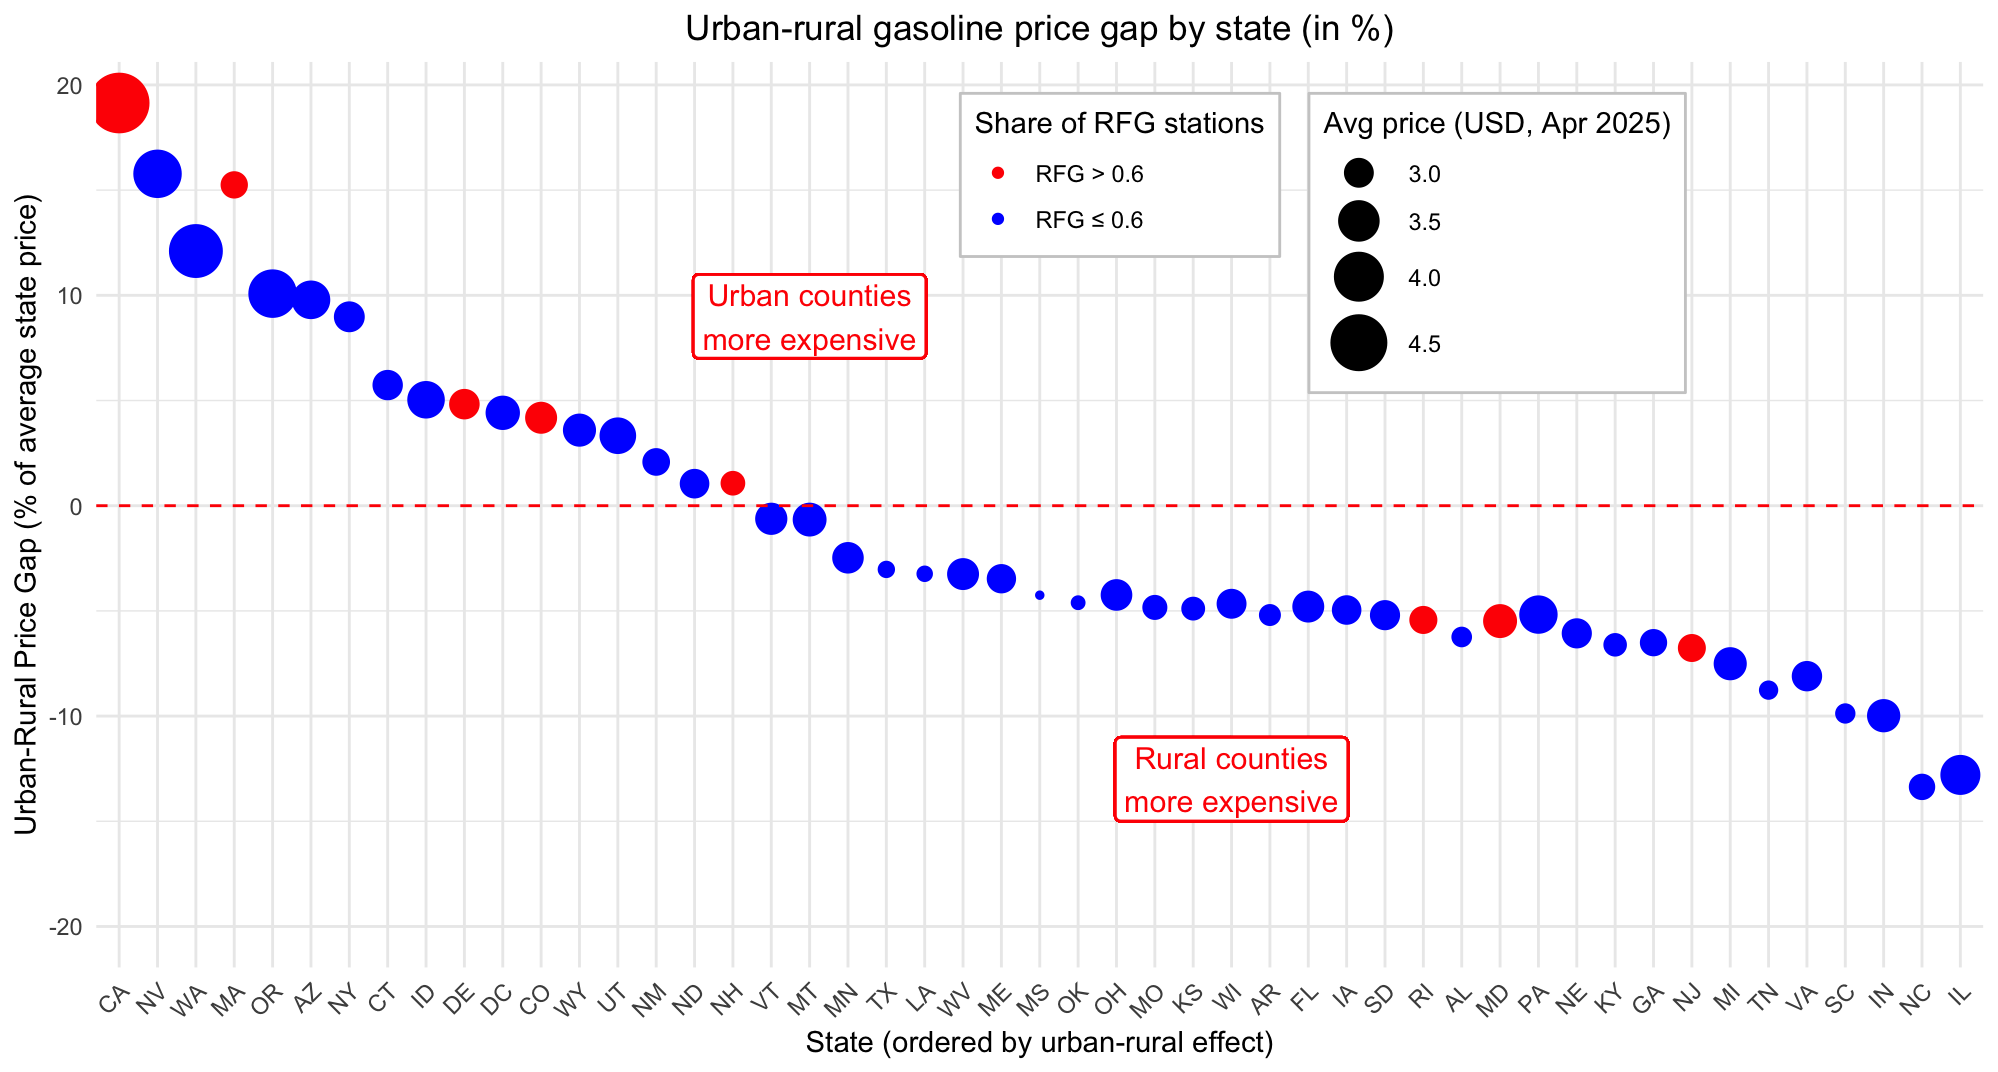
\includegraphics[width=\linewidth]{Figures/Rplot02.png}
\caption{State-Level Urban–Rural Gasoline Price Gaps (as Percentage of State Average)}

    \label{fig:Figure2}
\end{figure}

\newpage
% \label{figure}


\newpage

\bibliographystyle{apalike}
\bibliography{Bibliography}


\end{document}